\RequirePackage{ifpdf}
\ifpdf
\documentclass[12pt,            % 11pt Font
               a4paper,         % a4-Paperformat
               twoside,         % twoside 
%%             fleqn,           % Equations appear flush left
%%             draft,
               pdftex
               ]{book}
\else
\documentclass[12pt,            % 11pt Font
               a4paper,         % a4-Paperformat
               twoside,         % twoside 
%%             fleqn,           % Equations appear flush left
%%             draft,
%%               openright        % Chapters begin on odd (right) page
              ]{book}
\fi

\textwidth  450pt  
\oddsidemargin 3mm
\evensidemargin 8mm
%\evensidemargin 5mm

%\baselineskip 10mm
\textheight 580pt
%\parindent 5mm

%\renewcommand{\baselinestretch}{1.55} %spaziatura 


\ifpdf
 \usepackage[pdftex]{graphicx}
 \usepackage{pdflscape}
\else
 \usepackage[dvips]{graphicx}
 \usepackage{lscape}
\fi

\usepackage{url} 

\usepackage{ae} 
\usepackage{color}
\ifpdf
 \usepackage{pdfpages}
 \usepackage[colorlinks,plainpages=false]{hyperref}% generates colored links
\fi

\usepackage[small,bf]{caption}    

\newcommand{\TiberCAD}{{{T{\scriptsize IBER}CAD}}}
\newcommand{\tibercad}{\TiberCAD}
\newcommand{\Models}{\texttt{Models}}
\newcommand{\Device}{\texttt{Device}}
\newcommand{\Region}{\texttt{Region}}
\newcommand{\Simulation}{\texttt{Simulation}}
\newcommand{\physicalmodel}{\texttt{physical\_model}}
\newcommand{\keyword}[1]{\texttt{#1}}
\newcommand{\rvec}{{\bf r}}
\newcommand{\eps}{{\varepsilon}}

\usepackage{amsthm,amsmath}
\theoremstyle{plain}

\usepackage{float}

%\floatstyle{boxed}
\newfloat{code}{htp}{lop}
\floatname{code}{Listing}
\newenvironment{inputfile}{\begin{code}\begin{center}\begin{minipage}{0.8\textwidth}\rule{\textwidth}{0.1pt}}{\rule{\textwidth}{0.1pt}\end{minipage}\end{center}\end{code}}
\newcommand{\inputref}[1]{Listing~\ref{#1}}


\begin{document}

\ifpdf
 \DeclareGraphicsExtensions{.jpg, .png, .pdf}
\else
 \DeclareGraphicsExtensions{.eps}
\fi



\title{T{\large IBER}CAD User Manual}
\author{Fabio Sacconi, Matthias Auf~der~Maur, \\ Michael Povolotskyi, Giuseppe Romano } 
\maketitle


\pagenumbering{Roman}

\ifpdf\phantomsection\fi
\addcontentsline{toc}{chapter}{Contents}
\tableofcontents
%\listoffigures
\newpage 
%\pagestyle{fancy}

%\headsep 50pt
                               
\pagenumbering{arabic}



\chapter{Overview}




\section{Intoduction to numerical simulation with TiberCAD{} }

TiberCAD{} is  a multiphysics software tool; it  comprises  a  set  of  solvers, called   simulation models, each one describing a physical problem to be solved, e.g. DriftDiffusion (to solve Poisson and DriftDiffusion equations), EFASchroedinger (to solve Schroedinger equation in envelope function  approximation), Macrostrain (to calculate macroscopical strain with an elastic model) and others.

Similarly to  other device CADs, TiberCAD{} requires that one follows
 a three-step procedure.

 In a first step the device geometry must be sketched, giving all the geometrical information needed by the simulations. This can be performed by means of a   text file or with the help of a graphical tool.
During  this  procedure one or more {\em mesh regions} and {\em boundary  regions} have  to  be  defined: in a following stage the  {\em mesh regions} will  be  associated to  materials and {\em boundary  regions} to device  contacts (boundary  conditions  in  general).
 %The main output of this procedure is a geometry file that specifies one or more {\em mesh regions}. 

The second step consists in running a {\em mesher} tool, which reads the geometry file and sets up the computational mesh used to discretize the partial differential equations representing the physical models to be solved. For this procedure \tibercad  makes use of the GPL software {\em gmsh}. 
Optionally, mesh outout provided by other meshers, such as the one included in  ISE-TCAD tool, are also supported. 
The output of the meshing  procedure is a mesh file that contains information about the space discretization as well as the {\em mesh regions} and the {\em boundary  regions}. 

In the last step the actual simulations are performed. Together with the mesh information (comprised in the  mesh file ), TiberCAD{}  requires an input file which associates {\em materials} to {\em mesh regions}, defines the physical properties and physical models to be applied, and the type of calculations to be performed. 

Details about the modeler and mesher tools can be found in the specific user-manuals. Here we deal primarily with the TiberCAD{}   input file. However, in discussing examples of 1D, 2D and 3D simulations, we will also describe in some detail the geometry input files used to run {\em gmsh}.  
\subsection{ Input file  structure}
%The  execution of  the  requested  simulations  is  controlled  by  a  an  input file ,  e.g.  input.tib 
 TiberCAD{}   input file is  a  text file  which  includes  a  description of  the  device  structure,  the  definition of  the  solvers  to  be  executed,  with  all  the  relevant  physical and  numerical  parameters for  each  of  them.


The input file is organized into several sections, each describing a different aspect of the problem to be solved. The strategy employed is similar to other commercial T-CAD tools and requires some practice to reach a good level of familiarity. We strongly suggest to read first the following chapters (Getting  Started  1 and  2)  in this manual and then study the input files provided in the examples directory and try to  modify them, before writing your own  input file from scratch. The example files touch all current features implemented in the code.

Let's see  an  overview  of  the  main  features of the  input file 
The core of  the input file comprises three sections, called \textbf{Device}, \textbf{Models} and \textbf{Simulation}:

\begin{verbatim}
$Device
{
	Region Si_channel
	{
		
		material= Si	
		doping = 1e16
	}
	Region gate_oxide
	{
		
		material= SiO2
	}
	...
	
}

$Models
{
  model driftdiffusion
  {
    simulation_name= dd
  }
  
  ...
  
}

$Simulation
{
	solve= dd
}
\end{verbatim}

The section \textbf{Device} is used to associate one or more mesh regions to a material and to a set of   physiscal properties such as doping concentrations, doping levels, etc.
 The section
\textbf{Model} is used to define the physical models to be solved. Each physical model can be applied to the whole  device, or to a set of regions of  the  device,  (defined in \textbf{Device}   section). 
Finally, \textbf{Simulation}  section states the type of calculation to  be  executed,  that is  the  \textit{simulation} to  be  \textit{solved}.
These  sections  will  be  described  in full details  in  the  following.

Besides these  main  sections, there  other  other  two,  called  \textbf{Solver} and  \textbf{Physics},  where  some  parameters can  be  set,  respectively  for the  numerical solvers and  for  the  physical  models.
The  aim  of  these  sections is  to  give  the user the  maximum  of  flexibility to  tune his/her  simulation.
Especially  regarding  the  Solver  case,  values  of  the  numerical  parameters  have  been already  tuned for  each  application and   should  be  modified only  by an  advanced  user. 




% One \textbf{simulation} is a particular set of equations, boundary conditions, physical parameters, solver parameters, which describes a physical problem to be solved by \TiberCAD{}.
% A valid \TiberCAD{} \textbf{simulation} must belong to one of the predefined \TiberCAD{} \textbf{simulation} \textbf{models}
% (see section \ref{section:models}).



% To create a \TiberCAD{} \textbf{simulation}, we first have to declare the \TiberCAD{} \textbf{model} class to which our simulation belongs: 
% 
% 
% \begin{verbatim}
% $Models
% {
%   model driftdiffusion
%   {
%     ...
% \end{verbatim}
% 
% Here, we declare that the simulation to be created will belong to the \textbf{model} class driftdiffusion (\textit{model driftdiffusion})
% In the next \textit{Options} block, we define the \textbf{name} of the \TiberCAD{} \textbf{simulation} (\textit{simulationname = }) and the \TiberCAD{} regions to which it will be applied ( e.g., \textit{physical\_regions = all}, where 'all' means the whole device) 
% 
% In general, several \TiberCAD{} \textbf{simulations} belonging to the same \textbf{model} can be created; each of them must have a different name.   As we will see in the following (see \ref{section:solver},\ref{section:physics}) , it is possible to specify physical and solver parameters for a single \TiberCAD{} \textbf{simulation}, by referring to its  \textbf{name}. Anyway, it is also possible to specify parameters \textbf{common} to all the \TiberCAD{} \textbf{simulations} belonging to the same \textbf{model}, by referring to the name of the \TiberCAD{} model instead (in this case \textit{'driftdiffusion' }).




\section{Definition of physical and boundary regions in  TiberCAD{} }

\label{overview_boundaries}

Let'see  now  in  more  detail how  to  associate  \textit{physical}  information to  the  regions  of  the  device  model and  how  to  define  the  boundary  regions,  that  is  contacts or, in general,  regions  where  some  kind  of  boundary  condition is  to be  applied.

When \TiberCAD{}  is  run,  it  reads  the  mesh  file which  contains  the finite element  grid  which meshes the  geometrical description of  the  device or  nanostructure,  and  which will be  the  basis of  PDE  discretization.


As we  have  seen  before, to  execute the  proper  simulations, \TiberCAD{} needs  some  information about  the   physical and boundary regions  associated with the  mesh.
A physical region associates all  the  elements  corresponding to  an  homogeneous  part  of  the  device (usually  related to  the  same  material or  doping).   In  \TiberCAD{}, these regions  are  referred to as \textbf{mesh\_regions}.
\
%\subsection{Definition of contacts: boundary regions in  TiberCAD{} }

As for boundary regions, they  are  needed to  specify   boundary  conditions (b.c.)  for  the  solution of  the PDEs  of  our  simulation.
By  default,  to all   the  external boundary  of  the  device  a  Neumann b.c. is  imposed,   meaning  null  derivative  of  electric  field  and  zero  flux  of  current  normal to  the  boundary.  These are  the  usual  b.c.  applied in  the   simulation  of  electronic  devices;  in   particular, these  conditions are  implicitly  satisfied by using  the  finite  element  formulation..
%
Usually,  however, one  needs  to  impose   also   specifical  b.c.  to  the  device,  relative,  most  often, to  contacts of  some  kind (ohmic, schottky),  but  also   heat and  temperature b.c.  or  reference substrates  for  strain  calculations.
These  regions,  (constituted by  surfaces, lines or  points,  respectively  for  3D,  2D  and  1D  simulations) are  called in  \TiberCAD{}  \textbf{boundary regions}.


It  is  important to  know  that  the  information about  the   physical and boundary regions  must  be  present in  the  mesh  file  before it  is  read  by  \TiberCAD{},  and  thus  have  to  be  produced by  making  use of  the  modeling/mesher  software.
As  for  now,  \TiberCAD{} supports  the  mesh  output  of  the  following   software tools:  \textbf{GMSH v.2} and  \textbf{ISE-TCAD  v.9.5}.

\subsection{Using ISE-TCAD }

By  means  of  the  utility DEVISE    of  ISE-TCAD  v.9.5,  it  is  possible  to  design and  mesh  a  device;  after the  meshing  has  been    successfully performed,  an  output  file is  produced,   with  the  extension  \textit{.grd}.
This  file  contains    the  description of  the  mesh and  also  the  list  of  the  user defined  material  regions    and  contact  regions.
By  reading  this  \textit{.grd} file  in  \TiberCAD{},  one  can  refer  to  the  ISE TCAD material  regions,  simply  with  the  user-defined name,  which is  present  in  the    \textit{.grd}  file.  This  name  should  be  unique in  the  whole  device.
In the  same way,  ISE TCAD Boundary regions (\textit{Contacts})  can  be  referred to in   \TiberCAD{}  by  means  of  their  user-defined name, present in  the   \textit{.grd} output  file,  too.

\subsection{Using GMSH }

If  GMSH  program  is  used  to  model and  mesh  the  device,  a  bit  more  care  has  to  be  taken. 
Here  we   introduce  the  procedure  to  be  followed; in  the  following tutorials  (Getting  started...  the  subject  will  be  considered  in detail  with  a  step-by-step  description.  
See also the GMSH user manual (\url{http://geuz.org/gmsh}) for  further  details. 

In  the  context of  GMSH,  it  is  possible to  define  several 1,  2  and  3D \textit{Physical Entities}.
These \textit{Physical Entities} allow  to  associate one or more  geometrical  entities to  a  single  numerical  ID
or, better, to  a string label,
so  that  several  
\textbf{mesh\_regions}  and  \textbf{boundary regions} can  be  defined and  referred  to  by  TiberCAD{}.  
Here is  a  simple example  of   a  script  to  generate a  1D geometrical  model ( \textit{*.geo})  file in  GMSH: (see also  chapter \ref{chap:Gettingstarted1D})

\begin{verbatim}
Point(1) = {-25,0,0,0.5};
Point(2) = {0,0,0,0.002};
Point(3) = {25,0,0,0.5};
Line(1) = {1,2};
Line(2) = {2,3};


Physical Line("p_side") = {2};
Physical Line("n_side") = {1};
Physical Point("cathode") = {3};
Physical Point("anode") = {1};
\end{verbatim}

Here,  first the   geometrical  entities  \textbf{Point}s  and  \textbf{Line}s  are  defined. 

In the definition of the geometrical \textbf{Points},  the three first expressions inside the braces on the right hand side give the three X, Y and Z coordinates of the point ; the last expression (0.5 or  0.002 in  this  example) sets the \textbf{characteristic mesh length} at that point, that is the \textbf{size} of a mesh element, defined as the length of the segment for a line mesh element, the radius of the circumscribed circle for a triangle mesh element and the radius of the circumscribed sphere for a tetrahedron mesh element.
Thus, the smaller is the value of the \textbf{characteristic mesh length}, the greater is the mesh density close to that point. The size of the mesh elements will
then be computed in GMSH by linearly interpolating these characteristic lengths in the whole mesh.

In the definition of a geometrical \textbf{Line},  the two expressions inside the braces on the right hand side  give the identification numbers of the start and end \textbf{Points} of the line.


 Then,  two  physical  regions are  defined, each  associated to  one  of  the  two  geometrical  entities:  \textbf{Physical Line(n\_side)}  and \textbf{ Physical Line(p\_side)}. 
The expression(s) inside the braces on the right hand side  give, in general, the identification numbers of all the geometrical lines that need to be grouped inside the \textbf{Physical Line}.

 In this  way,  these  physical  regions are made  available for  \TiberCAD{},  and  will be  used  to  associate them  to  a  \TiberCAD{} region through the  keyword \textbf{Region} ,  as  follows:
\begin{verbatim}
Region n_side
   {
     ............

............

Region  p_side 
   {
     .............

...........
\end{verbatim}


It  is also possible  to  group more than  one  physical region in a  single  Device  Region,  with the  keyword \textbf{mesh\_regions},  as  follows:


\begin{verbatim}
Region reg_1
   {
     mesh_regions  = (region1, region2)

............

Region  reg_2
   {
     mesh_regions  = (region3, region4)

...........
\end{verbatim}

Note  that, in  this case, \textit{region1, region2, region3, region4}  are  the  labels  previously  defined inside  GMSH,  while  \textit{reg\_1 and  reg\_2} are  names chosen  by  user for  his  convenience.


Then,  in  the  GMSH  script,  two  \textbf{Physical Point }  are  defined, \textbf{anode}  and \textbf{ cathode},   and  associated to  the  first  and  to  the   last  point  of  our  1D  device.  These  points  are  needed  to  impose  some  boundary  conditions   and  in this  way  they  are made  available for  TiberCAD{},  and  will be  used  to  associate each  of  them  to  a  boundary  condition  region, through the  keyword 
\textbf{BC\_Region}:

\begin{verbatim}
BC_Regions  
    {
      BC_Region cathode
      {
        .........

......................

	BC_Region anode
        {
          ........

....................

\end{verbatim}

As  before,  it  is  possible  group more  boundary regions in  a  single \textbf{BC\_Region}, with  the  keyword 
 \textbf{BC\_reg\_numb}

\begin{verbatim}
BC_Regions  
    {
      BC_Region cathode
      {
        BC_reg_numb = (contact1,  contact2)

......................

	
....................

\end{verbatim}

Again,  in  this second  case,  \textit{cathode}  is  a  label  chosen  by user,  while  \textit{contact1} and  \textit{contact2} are    labels  previously  defined inside  GMSH.


In  2D  case,  a  set  of  \textbf{Physical Surface}  will  be  defined  to  be  used  as   \textbf{mesh\_regions},  while  
\textbf{Physical Line}  is  used  for  \textbf{boundary regions}.

Finally,  in  3D  case,  \textbf{Physical Volume} is   used  to  define  \textbf{mesh\_regions},  while \textbf{Physical Surface} is  used  to  define  \textbf{boundary regions}.




\section{Simulation  environments }

\TiberCAD{} allows  to  compute  different  physical models in  different parts of  a  device or  nanostructure by  coupling in a general way different  \textit{simulation  environments}.
 A \textit{simulation  environment} is  composed  by  all  the  physical regions to  which  a  particular model  is  assigned.
A \textit{simulation  environment} is  therefore  defined by  the  mesh  elements belonging to its physical regions and  by  the  \textbf{simulation model} which has  been  associated to  these  regions.
This  association is  made possible  by  the  definition of  \TiberCAD{} \textbf{Regions} and  \textbf{Clusters}.
Different   \textit{simulation  environments} can  have  physical regions  in  common.
In this  way,  each  simulation  is  run  on  a  subset  of  the  device  and  can  be possibly  coupled  (even self-consistently)   with  a simulation  run on  a  different subset  of  the  device corresponding to a \textit{simulation  environment} with a  non-void  intersection with  the  first  one.  The  coupling  of  the  two  simulations is  performed 
%at  the  boundary between  the  two  \textit{simulation  environments}, 
 by  means  of  appropriate  Boundary  Conditions (e.g. Current Density, Voltage, ...).
 In  principle, the  two \textit{simulation  environments}  can    refer to  two simulations at  different scale, e.g. atomistic  tight-binding  and  macroscopic drift-diffusion. This  allows an effective  \textbf{multi-scale} simulation of the  device to be  studied.

















\chapter{Getting  started 1D}
\label{chap:Gettingstarted1D}
In this  section we  will  see,  step by  step,  how  to use  \TiberCAD{} to simulate numerically a  semiconductor  device.
As a very  simple example  we  will  refer  to  the  \textbf{Tutorial 0} (Si bulk) that you  can  find  in  the  \textit{Tutorials}  directory.



\section*{Step 1: Modeling the device}

As a first step, we have to model the device. To do so, you can use DEVISE module of ISE-TCAD 9.5 software package or GMSH program.
Here we'll see in details the procedure for GMSH.
There are two possible ways to use GMSH:

    
\begin{enumerate}
	\item Interactive, using the graphical interface
   \item Using a script file.
\end{enumerate}

In the following we'll see how to write a basic GMSH script (bulk.geo); for any details please refer to GMSH manual GMSH (http://geuz.org/gmsh/).

 

 

In a GMSH script, several variables can be defined and given a value in this way:

\begin{verbatim}
L = 1;
d = 0.01;
\end{verbatim}

these are valid GMSH variables: \textit{L} is just the length of the Si sample; \textit{d} is the value of a \textbf{characteristic}
\textbf{mesh length} (see below).
\begin{itemize}
	\item Definition of geometrical entities \textbf{Points}:
\end{itemize}


\begin{verbatim}
Point(1) = {0, 0, 0, d};
Point(2) = {L, 0, 0, d};
\end{verbatim}

In the definition of a geometrical point, the three first expressions inside the braces on the right hand side give the three X, Y and Z coordinates of the point ; the last expression \textit{(d)} sets the \textbf{characteristic mesh length} at that point, that is the \textbf{size} of a mesh element, defined as the length of the segment for a line segment, the radius of the circumscribed circle for a triangle and the radius of the circumscribed sphere for a tetrahedron.

Thus, the smaller is the value of \textit{d,} the greater is the mesh density close to that point. The size of the mesh elements will then be computed in GMSH by linearly interpolating these characteristic lengths in the whole mesh.

\begin{itemize}
	\item Definition of geometrical entity \textbf{Line}:
\end{itemize}
  
\begin{verbatim}
Line(1) = {1, 2};
\end{verbatim}
The two expressions inside the braces on the right hand side  give the identification numbers of the start and end points of the line.

\begin{itemize}
	\item Definition of the physical entity \textbf{Physical Line 1}:
\end{itemize}

\begin{verbatim}
Physical Line(1) = {1};
\end{verbatim}

The expression(s) inside the braces on the right hand side  give the identification numbers of all the geometrical lines that need to be grouped inside the \textbf{physical line}.
In this way, in general, \textbf{physical regions} are created which associate together geometrical regions, and then the related mesh elements, which share some common physical properties. It's only these physical regions which can be referred to outside GMSH. In \TiberCAD{}, this is done by associating one or more physical regions to a \textbf{TiberCAD{} region }through the keyword \textbf{mesh\_regions} (see in the following).

\begin{itemize}
\item Definition of two physical entities\textbf{ Physical Point}:  
\end{itemize}

\begin{verbatim}
Physical Point(1) = {1};
Physical Point(2) = {2}; 
\end{verbatim}

Beginning  from  GMSH v.2, it  is  possible, alternatively,   to  assign  more  convenient \textbf{Physical Names}  to  the  Physical entities, instead of  numerical IDs.  \textbf{Physical Names} consist of  strings  enclosed between  quotation marks.
The  syntax is the  following:

\begin{verbatim}
Physical Line("bulk") = {1}
............
Physical Point("Anode") = {1};
\end{verbatim}



    \textbf{N.B}.: In general, in a \textit{nD} simulation, \textit{(n-1)D }physical regions (points in 1D, lines in 2D, surfaces in 3D) are used by \TiberCAD{} to impose the required boundary conditions.
      Each  \textit{(n-1)D } physical region defined in this way in GMSH will be associated in \TiberCAD{} to a boundary condition region, through the keyword \textbf{BC\_reg\_numb}. Thus, in this case, Physical points \textbf{1} and \textbf{2} will be associated respectively to two BC regions (see in the following).






\section*{Step 2: Meshing the device}

The \textit{.geo} script file with the geometrical description can be run in GMSH, to display the modelled device and to mesh it through the GMSH graphical interface.
Alternatively, a \textit{non-interactive} mode is also available in GMSH, without graphical user interface. For example, to mesh this 1D tutorial in non-interactive mode, just type:

\textit{gmsh bulk.geo  -1 -o bulk.msh }

where \textit{bulk.geo}  is the geometrical description of the device with GMSH syntax;
\textit{-1} means 1D mesh generation;

some command line options are:

\textit{-1, -2, -3} to perform 1D, 2D or 3D mesh generation,

\textit{-o} mesh\_file\textit{.msh} to specify the name of the mesh file to be generated

In this way, a \textit{.msh} has been generated and is ready to be read in \TiberCAD{}. 





\section*{Step 3: TiberCAD{}  Input file  }

Now we have to write down the \TiberCAD{} \textbf{input file} (see \textit{bulk.tib} in  the  Tutorials).


\subsection* {1 - Definition of Device Regions}
First, we have to list all the \TiberCAD{} Regions present in our Device: a \TiberCAD{} \textbf{Region} is usually a section of the device featuring the same material and possibly the same doping.
\begin{verbatim}
$Device
{
Region bulk
{
mesh_regions = 1
material = Si
doping = 1e16 doping_type = donor
}

}
\end{verbatim}
The \TiberCAD{} \textbf{Region} bulk is made of Silicon and n-doped with a concentration $10^{16} cm^{-3}$ .

Through the keyword  \textbf{mesh\_regions} , one or more of the \textit{physical regions} (\textit{Physical Lines} in 1D, \textit{Physical Surfaces} in 2D, \textit{Physical Volumes} in 3D) previously defined in the GMSH mesh can be associated to the present  \TiberCAD{} \textbf{Region}.

With \textit{mesh\_regions = 1}, we associate the Physical Line 1, defined in the Step 1, to the \TiberCAD{} \textbf{Region} \textit{bulk}.

\subsection* {2 - Definition of Simulation}

Now we define the \textbf{Simulation} \textit{driftdiffusion\_1}: it belongs to  the class \textbf{driftdiffusion}
\begin{verbatim}
Models
{
model driftdiffusion
{
options
{
simulation_name = driftdiffusion_1
physical_regions = all
}
\end{verbatim}

The \TiberCAD{} \textbf{simulation} \textit{driftdiffusion\_1} , belonging to the  \textbf{model} \textbf{driftdiffusion}, will be applied to the whole device structure (\textit{physical\_regions = all}).


\subsection* {3 - Definition of Boundary Conditions}
The anode and cathode contacts of our 1D Si sample are defined as \textbf{Boundary conditions regions} (\textit{BC\_Region anode , BC\_Region cathode}) in the following way:

\begin{verbatim}
BC_Region anode
{
BC_reg_numb = 1
type = ohmic
voltage = @Vb
}

BC_Region cathode
{
BC_reg_numb = 2
type = ohmic
voltage = 0.0
}
\end{verbatim}
Both contacts are defined as \textit{ohmic}, cathod is assigned a fixed \textit{voltage = 0.0}, while anode voltage is given by the value of the variable \textit{Vb (voltage = @Vb)}.

Through the keyword  \textbf{BC\_reg\_numb} , one or more of the \textbf{(n-1)D} physical regions (Physical Points in 1D, Physical Lines in 2D, Physical Surfaces in 3D) previously defined in the GMSH mesh can be associated to the present  \TiberCAD{} \textbf{BC Region}.
With \textit{BC\_reg\_numb = 1}, we associate the Physical Point 1, defined in the \textbf{Step 1}, to the \TiberCAD{} \textbf{BC Region} \textit{anode}; with \textit{BC\_reg\_numb = 2}, we associate the Physical Point 2, defined in the \textbf{Step 1}, to the \TiberCAD{} \textbf{BC Region} \textit{cathode}.

Alternatively, one can make  use  of  the  \textbf{physical names} associated to the physical regions in the  meshing  tool.
In  this  case, we  simply associate the  \textbf{(n-1)D} physical region,  respectively  ``anode'' and  ``cathode'',  by  means  of  the  \TiberCAD{} \textbf{BC Region name}:

 \begin{verbatim}
BC_Region anode
{

type = ohmic
voltage = @Vb
}

BC_Region cathode
{

type = ohmic
voltage = 0.0
}
\end{verbatim}

Note that, in  this  case, the \TiberCAD{} \textbf{BC Region name} needs to  be  identical to  one of the  \textbf{physical names} defined during the  modeling of the  device  with   GMSH.



\subsection* {4 - Definition of Simulation parameters}

The variable \textit{Vb }is specified in the \textit{sweep} block, in the \textbf{Solver} section
\begin{verbatim}
 sweep
{
simulation = driftdiffusion_1
variable = Vb
start = 0.0
stop = 1
steps = 10
}
\end{verbatim}

In this way, the simulation \textit{driftdiffusion\_1} is performed for 10 ( \textit{steps = 10}) values of the anode voltage (\textit{variable = Vb}), between 0 and 1.

\subsection* {5 - Definition of Execution parameters}
In the \textbf{Simulation} section , we decide \textit{which} simulations to perform and in which \textit{order}; we set
\textit{solve = sweep}, to execute the \textit{sweep} which run \textit{driftdiffusion\_1} \textbf{simulation} for the specified loop.
\begin{verbatim}
  $Simulation
{
#searchpath = .
meshfile = bulk.msh
dimension = 1
temperature = 300
solve = sweep
resultpath = output
output_format = grace
plot = (Ec, Ev, ContactCurrents)
}
\end{verbatim}
Output files with conduction and valence band profiles (\textit{plot = Ec,Ev.}.) and all the calculated values of the current at the contacts (\textit{ContactCurrents}) (the IV characteristic) are generated.



\section*{Step 4: Run TiberCAD{}}

Now we can run TiberCAD{}:

\texttt{tibercad  bulk.tib}


\vspace{0.5cm}
The generated \textbf{Output} files are:



\textbf{driftdiffusion\_materials.dat}: \textit{material} (mesh) regions, in this case just region 1

\textbf{driftdiffusion\_nodal.dat}: \textit{nodal} quantities (here conduction and valence band)

\textbf{sweep\_driftdiffusion\_Vb.dat} : \textit{integrated current} at the two contacts for each sweep step.



















%
%
% ***********************************************************************
%
%

%  Getting_started 2



\chapter{Getting  started 2D}


In this  second  example  we  will  refer  to  the  \textbf{Tutorial 4} (Si n-Mosfet) that you  can  find  in  the  \textit{Tutorials}  directory.



\section*{Step 1: Modeling the device}

Again, as a first step, we have to model the device. 

We'll see in some details how to design and mesh a mosfet device with GMSH.


\begin{itemize}
\item 
In the  GMSH script  \textit{mosfet.geo} , several variables are  defined and given a value in this way:                                                 \end{itemize}


\begin{verbatim}
lsub=0.03;
lacc=0.002;
lct=0.0005;
lg=0.0015;
lh=0.01;
lc=0.0005;
\end{verbatim}

these variables are used in the script to assign proper values to the \textbf{mesh characteristic lengh} of the defined Points 

\begin{verbatim}
Lg_2 = 0.0375;
d = 0.01;
Ls = 0.1;
h = 0.25;
b = 0.0025;
o = 0.005;

xd = Lg_2 + d;
xd2 = Lg_2 + d / 2;
xmax = xd + Ls - d;
\end{verbatim}
These other convenient variables are used to parametrize the most relevant geometrical features, such as channel length, oxide thickness,  and  so on. 


\begin{verbatim}
Point(1) = {0, -h, 0, lsub};
Point(2) = {0, 0, 0, lc};
Point(3) = {xmax,-h,0.0,lsub};
Point(4) = {-xmax,-h,0.0,lsub};
Point(5) = {xmax,0,0.0,lh};
Point(6) = {-xmax,0,0.0,lh};
..........................
Line(1) = {4,1};
Line(2) = {3,13};
Line(6) = {4,14};
Line(7) = {10,9};
Line(8) = {12,2};
Line(9) = {8,7};
Line(10) = {11,8};
Line(11) = {9,12};
Line(13) = {7,6};
..........................
\end{verbatim}

\begin{itemize}
\item 
Geometrical \textbf{Points} and \textbf{Lines} are  defined to design the device  structure; the  fourth parameter in \textbf{Point} assignement is  the   characteristic length associated to that point: this  is  an  essential feature to control the  mesh density and refine it where  necessary (usually n the channel region).     \end{itemize}

 

\begin{verbatim}
Line Loop(40) = {28,2,-34,33,8,29,-31,-30,-6,1};
Plane Surface(41) = {40};
..........................
\end{verbatim}
\begin{itemize}
\item 
Definition of a surface: first a \textbf{line loop} is composed, listing all the  lines constituting the  boundary of the surface; then this  line  loop is  assigned to a  \textbf{Plane Surface} object (this  procedure can be alternatively performed throgh the  graphical interface).                       \end{itemize}                                                                                                                                                                                                                             



\begin{verbatim}
Physical Surface(1) = {41}; // n-Si
Physical Surface(2) = {44,47}; // n+-Si
Physical Surface(3) = {46}; // SiO2
\end{verbatim}
\begin{itemize}
\item 
Definition of  the \textbf{Physical surfaces} : each of them is composed by one or more geometrical \textbf{Plane Surface}. For example, \textbf{Physical surface} 2 comprises the two separated contact regions, while \textbf{Physical surface} 3 corresponds to the  oxide  region.

The  \textbf{Physical surfaces} are the 2D Physical regions of  the  mesh and will  be  assigned to the related \TiberCAD regions through the keyword \textit{mesh\_regions}  (see   Step  )                                                                                                                   \end{itemize}                                                                   


\begin{verbatim}
Physical Line(1) = {13}; // source
Physical Line(2) = {39,38}; // gate
Physical Line(3) = {19}; // drain
\end{verbatim}
\begin{itemize}
\item 
Definition of the  \textbf{Phisical Lines}: In this 2D simulation, 1D physical regions are used to carry information about boundary condition regions. In  other word, each \textbf{Phisical Line} corresponds to a boundary condition (a contact in the case of a driftdiffusion calculation): thus Physical Line 1 refers to source contact, P.L. 2 to gate contact, P.L. 3 to drain contact.
The numerical identifications of these \textbf{Phisical Lines} will be  asigned to \TiberCAD \textbf{BC regions} by means of the \textit{BC\_reg\_numb} instruction.
\end{itemize}

In fig.  \ref{geo}  the  obtained  geometrical  model is  shown.


\begin{figure}
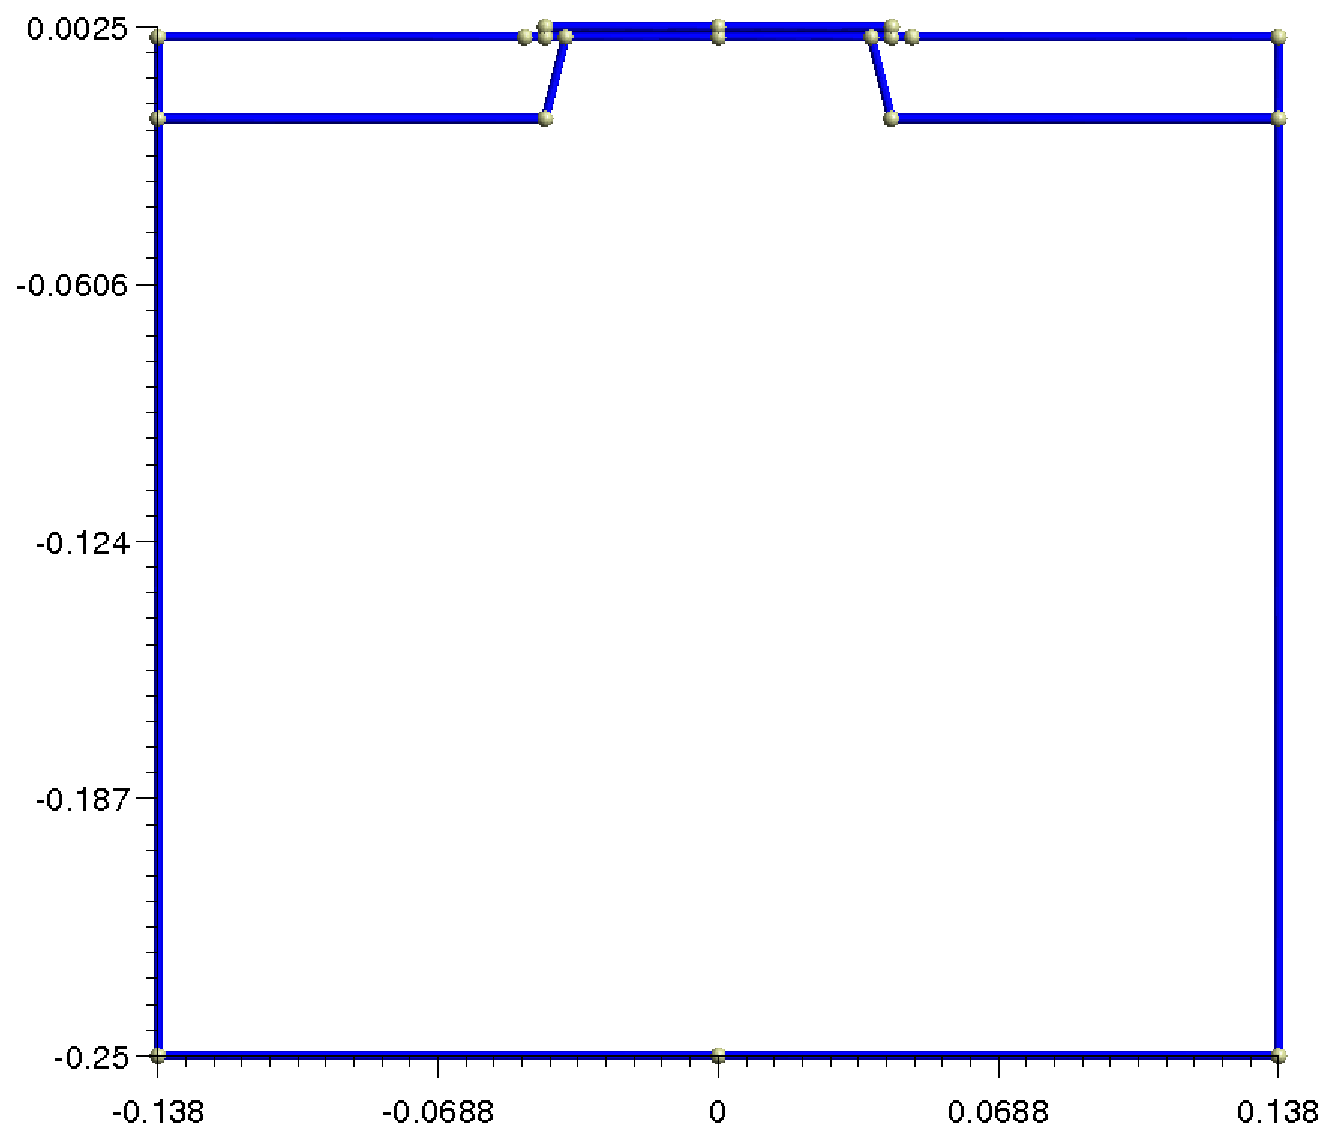
\includegraphics[width=8cm]{./figures/geomosfet}

%\centerline{
\psfig{figure=geomosfet.ps, angle = 270,width=9cm }}
\caption{Geometrical structure as  defined by GMSH modeller}
\label{geo}
\end{figure}
 


\section*{Step 2: Meshing the device}

The \textit{.geo} script file with the geometrical description can be run in GMSH, to display the modelled device and to mesh it through the GMSH graphical interface (see fig. \ref{meshmos}).
Alternatively, a \textit{non-interactive} mode is also available in GMSH, without graphical user interface. For example, to mesh this 2D tutorial in non-interactive mode, just type:

\textit{gmsh mosfet.geo  -2 -o mosfet.msh }

\begin{figure}
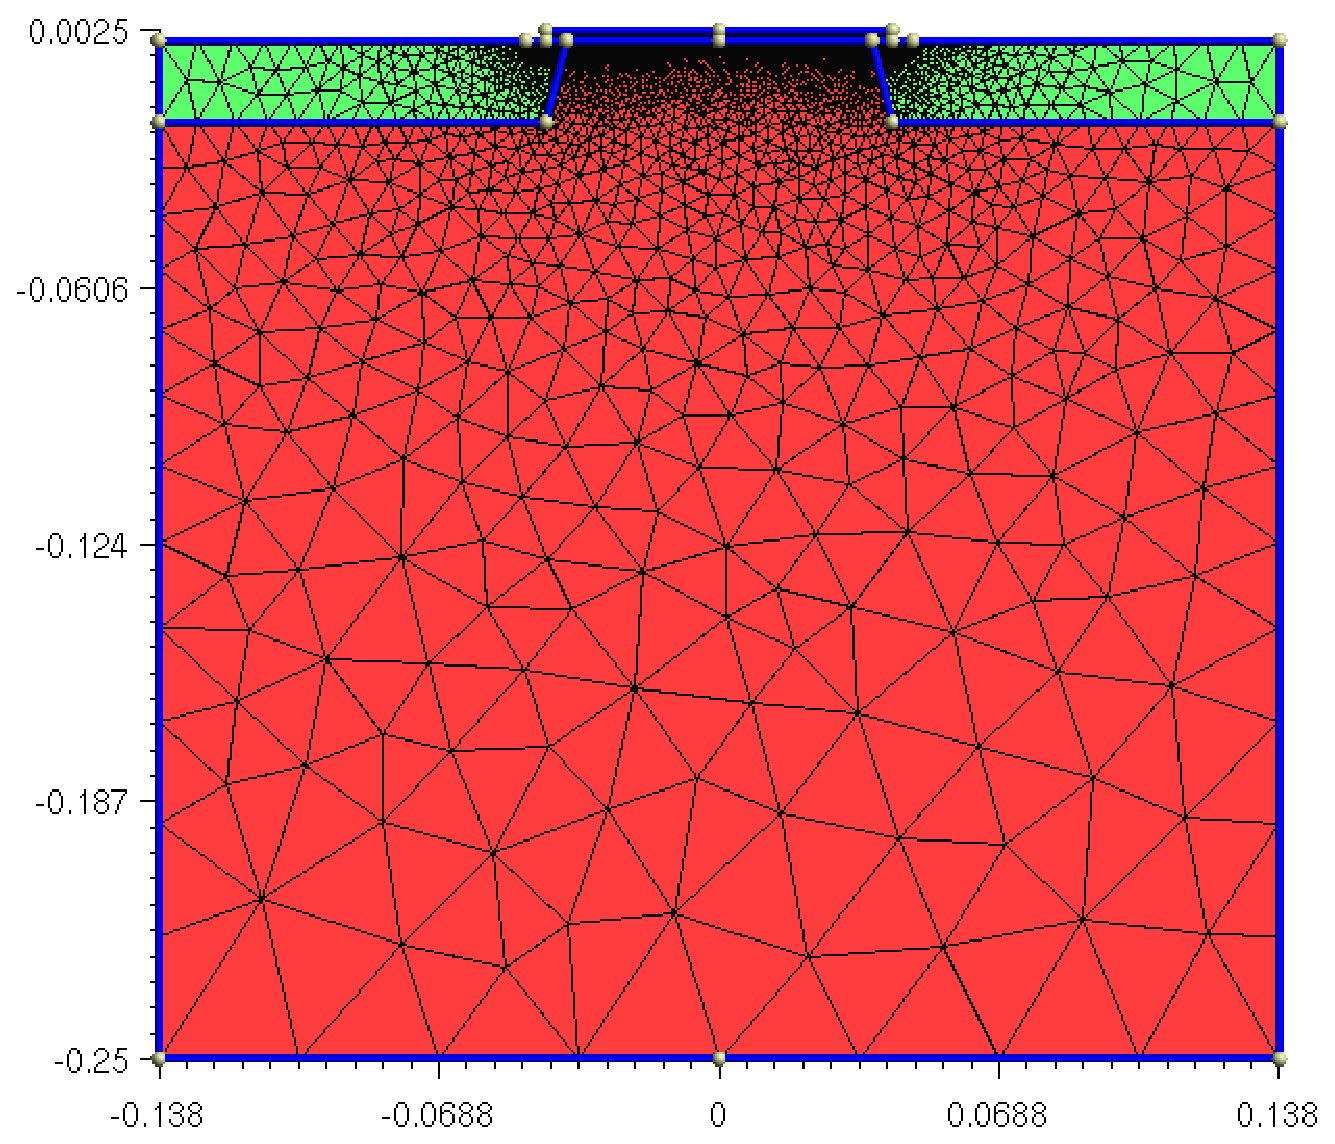
\includegraphics[width=8cm]{./figures/meshmosfet}

\caption{2D Mesh for the mosfet device obtained with   GMSH }
\label{meshmos}
\end{figure}




\section*{Step 3: TiberCAD  Input file  }

Now we have to write down the \TiberCAD \textbf{input file} (see \textit{mosfet.tib} in  the  Tutorials).


\subsection* {1 - Definition of Device Regions}

Three  \TiberCAD regions are  defined: to each of them, one  mesh\_region is  associated, that is the Phisical Surfaces  \textbf{1, 2} and  \textbf{3} defined in  Step 1. However, in general more than one  mesh\_region can be  associate to a single \TiberCAD region, if this is convenient.

\begin{verbatim}
 Region substrate 
   {
     mesh_regions = 1
     material = Si
     doping = 1e18 doping_type = acceptor
   }
   
   Region contact
   {
     mesh_regions = 2
     material = Si
     doping = 5e19 doping_type = donor
   }

   Region oxide
   {
     mesh_regions = 3
     material = SiO2
  
   }

\end{verbatim}


\subsection* {2 - Definition of Simulation}

Now we define the \textbf{Simulation} \textit{dd}: it belongs to  the class \textbf{driftdiffusion}

\begin{verbatim}
   model driftdiffusion
  { 
              
    options
    {
     simulation_name = dd
     physical_regions = all
    }


\end{verbatim}

We declare two \textbf{driftdiffusion physical models}:
 the  first defines a   \textit{srh} \textbf{recombination}  model (see \ref{dd:recomb_models}); the  second 
defines a \textit{field-dependent} \textbf{mobility} model for  electrons which implements a \textit{doping  dependence} for the \textbf{low-field  mobility} (see \ref{dd:mobility_models}).

% respectively about \textbf{mobility} (\textit{field\_dependent}) and  \textbf{recombination} (\textit{srh});  see  the reference manual  for  the  details \ref{dd:recomb_models}, \ref{dd:mobility_models}

\begin{verbatim}

    physical_model recombination
    {
      model = srh
    }

    physical_model electron_mobility
    {

      model = field_dependent
      low_field_model = doping_dependent   

    }



\end{verbatim}

\subsection* {3 - Definition of Boundary Conditions}
The source, drain  and gate contacts of the Mosfet device  are defined as \textbf{Boundary conditions regions} (\textit{BC\_Region source , BC\_Region drain, BC\_Region gate }) in the following way:

\begin{verbatim}
    BC_Region gate
      {
        BC_reg_numb = 2
        type = schottk
        barrier_height = 3.0
        voltage = @Vg[0.0]
      }

      BC_Region source
      {
        BC_reg_numb = 1
        type = ohmic
        voltage = 0.0
      }
 
      BC_Region drain
      {
        BC_reg_numb = 3
        type = ohmic
        voltage = @Vd[0.5]
      }


\end{verbatim}

To each of the  \textbf{BC regions}, one \textit{BC\_reg\_numb} is  assigned,  that  is  one  of the Physical Lines \textbf{1,2, 3} defined in \textbf{Step 1}, which represent the contact regions.

Note that, while \textit{source} and \textit{drain} are defined as \textit{type= ohmic},  \textit{gate} \textbf{BC region} is defined as \textit{type = schottky};
\textit{barrier\_height = 3.0} specifes the metal/oxide interface barrier and depends on the contact metal workfunction.

Drain voltage is defined as \textit{@Vd[0.5]} and  gate voltage as \textit{@Vg[0.0]}. This specifies that the value of the voltage will be  determined at each moment of the simulation, by the value of the two variables \textit{Vd} and \textit{Vg}, which will be assigned in the \textbf{sweep}  definition. 

 
\subsection* {4 - Definition of Simulation parameters}

Two sweeps are requested for this simulation, that is an external loop on \textit{Vg} (the gate voltage) and an internal loop on \textit{Vd} (the drain voltage) for each value of \textit{Vg}; in this way, the IV drain characteristics for a series of gate biases are obtained in output.

\begin{verbatim}
    sweep_1
  {
    simulation = dd
    variable = Vd
    start = 0.0
    stop = 2.0 #0.1
    steps = 200  #200 #1
 #   plot_data = true
  }

  sweep_2
  {
    variable = Vg
    start = -0.1
    stop = 0.5
    steps = 6
    simulation = sweep_1
    #simulation = driftdiffusion
  }


\end{verbatim}


\subsection* {5 - Definition of Execution parameters}

In the \textbf{Simulation} section , we decide    the  simulation dimension  (\textit{dimension = 2}), then \textit{which} simulations to perform
 and in which \textit{order}; we set
\textit{solve = sweep\_2}, to execute the external  gate  voltage sweep \textit{sweep\_2} which in  its  turn  call the sweep \textit{sweep\_1}  where drain current is  calculated for all the  chosen  drain voltage  steps by running   \textit{dd} \textbf{simulation}.

\begin{verbatim}
$Simulation
{
   meshfile = mosfet.msh
  dimension = 2
  temperature = 300
  solve = sweep_2 
  resultpath = output_IV_char 
  output_format = vtk
  plot = (Ec, Ev, QFermi_e, QFermi_h, eDensity, hDensity, eCurrent, hCurrent, 
          NetRecombination, EField, ElPotential, ContactCurrents)
}

\end{verbatim}

Output files with conduction and valence band profiles, quasi-fermi levels, electron and hole  density, recombination, electric field and potential (\textit{plot = Ec,Ev,....}.) will be  generated, together (\textit{ContactCurrents}) with  a file with  all the calculated values of the drain current at the contacts for each  gate bias  step  (the IV characteristics).

\section*{Step 4: Run TiberCAD}

Now we can run TiberCAD:

\texttt{tibercad  mosfet.tib}


\vspace{0.5cm}
The generated \textbf{Output} files are:

\textbf{driftdiffusion\_materials.vtk}:  information about the material regions of the device.

\textbf{driftdiffusion\_nodal.vtk}   output for the nodal quantities which have been calculated, e.g. conduction and valence bands, (quasi)fermi levels, electron and hole density and mobility.

\textbf{driftdiffusion\_elemental.vtk}  output for the elemental  quantities (e.g. electric field, current density).


\textbf{sweep\_2\_driftdiffusion\_Vg\_0.000\_Vd.dat}  and  similar for  all the  \textit{Vg}  steps: drain current characteristics for each \textit{Vg} bias.







\chapter{Input  file. }

Input for  \TiberCAD is  composed by an  input  file e.g. "input.tib" and a mesh file generated by a mesher software: as for  now, mesh files from GMSH (*.msh,  v.1)  and from ISE-TCAD (*.grd) are  supported.



A valid  input file is a  text file with the  following  structure.
  
It is composed by several sections:
%
each \textbf{section} begins with a section-name preceded by \char`\"{}\$\char`\"{} (e.g. \$Physics ).
A section is enclosed between  \char`\"{}\{\char`\"{} and \char`\"{}\}\char`\"{} brackets and is composed 
 by a number of  blocks enclosed between  \char`\"{}\{\char`\"{} and \char`\"{}\}\char`\"{} brackets.
   Each  \textbf{block} can be possibly composed by one or more blocks, each preceded by a block-name. 
 Everything following a '\textbf{\#}' is considered as a comment and is disregarded.

A parameters-block is  an elementary block which can contain 
%Except the model-blocks and the BC\_\-regions-blocks (see in the following), each block can contain 
zero or any number of   parameter assignements in the  form:

 \char`\"{}\textit{tagname} = \textit{tagvalue}\char`\"{}, where \char`\"{}\textit{tagname}\char`\"{} is a string and \char`\"{}\textit{tagvalue}\char`\"{} is a single numerical or string item or a list of items between \char`\"{}(\char`\"{} and \char`\"{})\char`\"{} parenthesis. Format is free for these assignements, provided they are separated by spaces. Everything which follows a '\textbf{\#}' is considered as a comment and is disregarded.
 Here and in the whole input file a string item can include a combination of characters, special characters and numbers, but not spaces; if a space is found , the string item is taken as terminated.
 
  
%List  of  keywords:

The input file is composed by  the following sections:

 \textbf{Device}  ,   \textbf{Models}  ,  \textbf{Physics},  \textbf{Solver},   \textbf{Simulation} 

%\textit{Models}:  driftdiffusion , thermal  ,  excitontransport,  macrostrain,   sweep(special)

\section{Device section }
%\textbf{Device} section:
\begin{verbatim}
$Device
{
 Region buffer
   {
   .........
   }
 Region barrier_1
   {
     ............
   }
   .................
}


\end{verbatim}





  In \char`\"{}\textbf{Device}\char`\"{} section, each block (Region-block) must be preceded by the keyword \char`\"{}\textbf{Region}\char`\"{}, followed by the  (single-word) name of the physical region.
For an ISE  mesh it must  be  the  same name defined during the  modeling of the  device.

\begin{verbatim}
   Region QWell
   {
     reg_numb = 4
     structure = wz
     y-growth-direction = (1,0,-1,0)
     z-growth-direction = (-1,2,-1,0)
     x-growth-direction = (0,0,0,1)
     mat = GaN
     doping = 1e17 doping_type = donor doping_level = 0.025
   }
\end{verbatim}
%The following keywords must always be  present in the body of each Region-block:  mat, reg\_numb .
%Other keywords  are optionals.
Here are the  description of  the available keywords for a Region-block.

%In the  header of  each block:
%\textit{Region} :   name of the  region; for ISE grid mesh it should  be  the  name defined during the  modeling of the  device.

%In the  body of the  block:

\textit{mat} (mandatory) :  name  of the  material associated to the  present region; it  can be  an  alloy,  in this  case the  keyword \textit{x } must be  present.

\textit{x} : alloy concentration; e.g. in $Al_xGa_{1-x}As$,  x is  Al concentration

\textit{ reg\_numb} (mandatory) : region ID as  specified in the meshing  program (GMSH).

\textit{structure} : crystal structure ( wz = wurtzite,  zb =  zincblend)

\textit{x-growth-direction}, \textit{y-growth-direction}, \textit{z-growth-direction}: Bravais  vectors with Miller  indexes for  wurtzite crystal (4 element vectors) or zincblende crystal  (3 element vectors).

\textit{doping} : doping  concentration [cm$^{-3}$]

\textit{doping\_type} : donor or  acceptor

\textit{doping\_level}: energy level of  the dopant [eV]


\section{Models section }



\begin{verbatim}
$Models
{ 
 model driftdiffusion
  { 
   ..........
   BC_Regions  
    {
      BC_Region cathode
      {
       ............
      }
      BC_Region anode
      {
        ..............
      }
    }   
  } 
 model macrostrain
  { 
  ...........................
 
\end{verbatim}




   In \char`\"{}\textbf{Models}\char`\"{} section, one or more  model-blocks must be present: each model-block must be preceded by the keyword \char`\"{}\textbf{model}\char`\"{}, followed by the (single-word) model name. 
 This must be the   name of  one of the  \TiberCAD  simulation models.
 
Here are the simulation models implemented until now:  \textbf{driftdiffusion} , \textbf{thermal}  ,  \textbf{excitontransport},  \textbf{macrostrain}.
   
   Each model-block can  contain the following optional blocks:
   
 %  one or more optional Boundary Condition regions blocks (\textbf{BC\_\-regions}-block).
   
   
 %   \char`\"{}\textbf{Models}\char`\"{} section can contain also 
   
\begin{itemize}
	
   \item one    "`options"' block, preceded by the keyword \char`\"{}\textbf{options}\char`\"{}. This block can contain    general  options for the present  model.
	\item  one or more  \textbf{physical\_model} blocks: each physical\_model block must be preceded by the keyword \char`\"{}\textbf{physical\_\-model}\char`\"{}, followed by the (single-word) name of the physical model.
	Each physical\_model block can contain parameters  relevant to a specifical model of a physical property or quantity related to the present model.
\item    one or more  Boundary Condition regions blocks (\textbf{BC\_\-regions}-block).
   The BC\_\-regions-block must be preceded by the keyword \char`\"{}\textbf{BC\_\-Regions}\char`\"{} and it is composed by one or more parameters-blocks, each preceded by the keyword \char`\"{}\textbf{BC\_\-Region}\char`\"{} followed by the (single-word)  name of the boundary condition region. This parameters-block can contain the possible description of the boundary region.
\end{itemize}


 
A detailed description of the possible parameters for these blocks  follows.



\subsection{options block }

\begin{verbatim}
options
    {
     simulation_name = driftdiffusion
     physical_regions = all
    }
\end{verbatim}

\textit{simulation\_name}: user-defined name of the particular instance of  the simulation model defined for this block. More than one simulation (with different  name and properties) can be  defined,in separated model blocks, which refer to a same  \TiberCAD  simulation model. If simulation\_name is  not assigned,  by default the \TiberCAD model name is taken as current simulation\_name.

\textit{physical\_regions}: (list of) physical region(s) to  which the  present simulation model will be  applied.
Physical region(s) can be integer numbers, consistent with the physical regions set assigned through GMSH, or strings, corresponding to the  region names defined in ISE grid  file.
Default value  is  "`all"' (all  physical regions of the  device).



\subsection{physical\_model block }

\begin{verbatim}
    physical_model recombination
    {
      model = SRH
    }
\end{verbatim}


Currently available physical\_models and parameters:

\textbf{recombination}:

\textit{model}:  SRH,direct, exciton\_generation,  exciton\_dissociation

\textit{exciton\_simulation}: excitons


\textbf{electron\_mobility}

\textit{model}: doping\_dependent

\textbf{hole\_mobility}

\textit{model}: doping\_dependent



\subsection{BC\_region block }

\begin{verbatim}
 BC_Region anode
      {
        BC_reg_numb = 2
        type = ohmic
	      voltage = 0.0
      }
\end{verbatim}



%For each BC\_region:

\textit{BC\_region}: name of the  present boundary  region

\textit{ BC\_reg\_numb}:  BC region ID(s) as  specified in the meshing  program (GMSH).

\textit{ type}: type of  boundary condition: ohmic,  schottky,...  ,  substrate (for strain calculations).

\textit{ voltage}:  value of voltage [V] applied to the present BC region (for ohmic and  schottky BCs).

\textit{ zero\_grad\_fermi\_h}, \textit{ zero\_grad\_fermi\_e}: if true set  Neumann b.c. to the fermi level in the b.c. region.

If \textit{type} is \textsl{substrate}:

\textit{material} : name of  material in the \textsl{substrate}  region. 

\textit{structure} : crystal structure ( wz = wurtzite,  zb =  zincblend)

\textit{x-growth-direction}, \textit{y-growth-direction}, \textit{z-growth-direction}: Bravais  vectors with Miller  indexes for  wurtzite.




\section{Solver section }

\begin{verbatim}
$Solver
{ 
 driftdiffusion
  {
    quasi_equilibrium = (cathode, anode)
    nonlin_max_it = 25
    nonlin_abs_tol = 1e-7
  #  nonlin_step_tol = 1e-3
    lin_max_it = 150
    ksp_type = gmres
    pc_type = composite
    #pc_type = ilu
    ls_max_step = 0.05
    #current_integration_method = rstf
  }
...................

\end{verbatim}

In this section one can  define the  setting parameters for  the numerical solvers: the section is organized in blocks, each one preceded by a block-name equal to one of the  user-defined simulation name. Solver parameters defined in each block refer to that particular simulation.

Two extra blocks can be  present:
\begin{itemize}
	
	
%\begin{verbatim}
% BC_Region anode
%      {
%        BC_reg_numb = 2
%        type = ohmic
%	      voltage = 0.0
%      }
%\end{verbatim}
%
	
   \item \textbf{sweep} block, preceded by the keyword \char`\"{}\textbf{sweep}\char`\"{}. This block  contains  the  setting for a set of  calculations applied to a boundary region (e.g. to a drain contact for the calculation of a IV characteristic).
   
   
%\begin{verbatim}
% BC_Region anode
%      {
%        BC_reg_numb = 2
%        type = ohmic
%	      voltage = 0.0
%      }
%\end{verbatim}

  \item  \textbf{selfconsistent} block , preceded by the keyword \char`\"{}\textbf{selfconsistent }\char`\"{}. In this block it is possible to define a self-consistent calculation based on two different simulation models (e.g. driftdiffusion and excitontransport).

\end{itemize}

Here are some of  the  parameters:

\textbf{quasi\_equilibrium:}

\textbf{nonlin\_max\_it}

\textbf{nonlin\_abs\_tol}

\textbf{lin\_max\_it}

\textbf{ksp\_type}

\textbf{pc\_type}

\textbf{ls\_max\_step}

\textbf{ls\_type}

\textbf{current\_integration\_method}


%sweep
\textbf{simulation} :  simulations to which sweep is  applied

\textbf{boundary}: boundary region to which sweep is  applied

\textbf{start} , \textbf{stop}, \textbf{steps} : sweep starts from \textit{start} value, is repeated  \textit{steps} times and stops in \textit{stop}

\textbf{plotvariable}

%% selfconsistent

\textbf{simulations} : simulations to be   executed in a self-consistent cycle. 

%thermal
\textbf{current\_simulation}  :    current simulation model used for  thermal  model

%macrostrain
\textbf{substrate} 




\section{Physics section }
In this section several physical parameters can be entered,  in  addition to or  overwriting  the material parameters present in the material files.
The section is organized in blocks, each one preceded by a block-name equal to one of the  user-defined simulation name. Physical parameters defined in each block refer to that particular simulation.

Here are some of the possible parameters:

\textbf{statistics} : FD

\textbf{model}: specification of generical drift-diffusion or  exciton transport  simulation.
Possible values: \textit{simple}, \textit{strained} ,  \textit{unstrained}.  

\textbf{tau\_rad}, \textbf{tau\_nonrad},  tau\_diss

\textbf{R}

\textbf{eff\_mass}

\textbf{mobility}

\textbf{generation\_model}



\section{Simulation section }

In this  section one  can  specify  several general parameters and settings  for  the  actual  calculation to be  run, such as the mesh file to be  used, the dimension of  simulation, the process-flow of  simulation, etc.

\textbf{searchpath} :  path for  material  files 

\textbf{meshfile} : name of  mesh file. N.B.: the extension is mandatory! ( .grd for ISE-TCAD, .msh for gmsh v.1 )

\textbf{mesh\_units} : units of  measurements used in the  meshing (relative to meters): e.g., $10^{-6}$ for  $\mu m$

\textbf{dimension} :  dimension of  simulation (1,2,3)

\textbf{temperature} :  temperature  of the system

\textbf{solve} : list of  simulations to  be  executed, in the order of  execution; if the list   contains "`sweep"', a sweep is  performed as specified in \textbf{sweep} block in the  \textbf{Solver} section.   

\begin{verbatim}
  solve =  (strain,driftdiffusion, quantum_electrons, quantum_holes)
\end{verbatim}



\textbf{resultpath} :  path for output  directory 

\textbf{output\_format} : format of  the  output data: \textbf{gmv},  \textbf{tecplot}, \textbf{grace} (for xmgr, ascii data column type),  ....

\textbf{plot} :  list of output variables which are calculated and available in output  files.


\chapter{Simulation of strain}
The theoretical model of strain simulation can be found in Refs.\cite{strain1, strain2}.
\chapter{Drift-diffusion simulation of electrons and holes}

\section{Theory}

The semi-classical transport simulation of electrons and holes is based on the drift-diffusion approximation (see e.g.~\cite{selberherr84}).

Beside the electric potential the electro-chemical potentials are used as variables such that the system of PDEs to be solved reads as follows
\begin{eqnarray}
-\nabla(\varepsilon\nabla\varphi - \mathbf{P}) & = & -e(n - p - N_d^+ + N_a^-) \nonumber \\
-\nabla(\mu_n n ( \nabla\phi_n + P_n \nabla T)  ) & = & R \\
-\nabla(\mu_p p (\nabla\phi_p + P_p \nabla T) ) & = & -R \nonumber
\end{eqnarray}
$P$ is the electric polarization due to e.g. piezoelectric effects and $R$ is the net recombination rate, i.e. recombination rate minus generation rate. $P_n$ and $P_p$ are the electron and hole thermoelectric power, respectively.
The models for the mobilities and the net recombination rates can be specified in the \texttt{physical\_model} sections as described in the following.


\section{Solution/Plot variables}

The solution variables available for plotting and for interaction with other models are given in Table~\ref{table:dd_solutions}.


\begin{table}[htb]
\center
\begin{tabular}{l|p{8cm}|l}
Key & Description & Units \\
\hline 
\texttt{Ec} & Conduction band edge & eV \\
\texttt{Ev} & Valence band edge & eV \\
\texttt{eQFermi} & Electro-chemical potential of electrons & eV ($-e\phi_n$) \\
\texttt{hQFermi} & Electro-chemical potential of holes & eV ($-e\phi_p$) \\
\texttt{Ec0} & Conduction band edge without electric potential & eV \\
\texttt{Ev0} & Valence band edge without electric potential & eV \\
\texttt{Eg} & Band gap & eV \\
\texttt{ConductionBands} & Minima of all conduction bands & eV \\
\texttt{ValenceBands} & Maxima of all valence bands & eV \\
\texttt{ElPotential} & Electric potential & V \\
\texttt{eDensity} & Electron density & cm$^{-3}$ \\
\texttt{hDensity} & Hole density & cm$^{-3}$ \\
\texttt{eMobility} & Electron mobility & cm$^2V^{-1}s^{-1}$ \\
\texttt{hMobility} & Hole mobility & cm$^2V^{-1}s^{-1}$ \\
\texttt{eConductivity} & Electron conductivity & S/cm \\
\texttt{hConductivity} & Hole conductivity & S/cm \\
\texttt{ElField} & Electric Field & Vcm$^{-1}$ \\
\texttt{Polarization} & Electric Polarization & Cm$^{-2}$ \\
\texttt{CurrentDensity} & Total current density & Acm$^{-2}$ \\
\texttt{eCurrentDensity} & Electron current density & Acm$^{-2}$ \\
\texttt{hCurrentDensity} & Hole current density & Acm$^{-2}$ \\
\texttt{IonizedDonors} & Ionized donor density & cm$^{-3}$ \\
\texttt{IonizedAcceptors} & Ionized acceptor density & cm$^{-3}$ \\
\texttt{IonizedElectronTraps} & Ionized electron trap density & cm$^{-3}$ \\
\texttt{IonizedHoleTraps} & Ionized hole trap density & cm$^{-3}$ \\
%\texttt{charge\_density} & Total charge density & cm$^{-3}$ \\
\texttt{eThElPower} & Electron thermoelectric power & V K$^{-1}$ \\
\texttt{hThElPower} & Hole thermoelectric power & V K$^{-1}$ \\
\texttt{NetRecombination} & %\begin{minipage}[t]{8cm}
%
%The net recombination rate for each recombination model and the total rate
%\end{minipage}& cm$^{-3}$s$^{-1}$
 The net recombination rate for each recombination/generation model and the total rate &
 cm$^{-3}$s$^{-1}$ \\
\texttt{ContactCurrent} & The electric current on each contact & A/cm$^{3-d}$
\end{tabular}
\caption{Solution/Plot variables}
\label{table:dd_solutions}
\end{table}


\section{Module options}

The following options influence the behaviour of the Drift-Diffusion module:

\begin{description}

\item[\keyword{coupling = }\Value{string}] defines which equations to solve. The default is \Value{full}, meaning that the full system consisting of the Poisson, electron continuity and hole continuity equations is solved. Other possible values are \Value{poisson} (for equilibrium calculations), \Value{electrons} or \Value{holes}. For the last two cases local equilibrium is assumed such that $\phi_n = \phi_p$.

%\item[\keyword{local\_equilibrium = }\Value{bool}] If \keyword{coupling} is set to \Value{electrons} or \Value{holes}, local equilibrium is assumed such that $\phi_n = \phi_p$. 

\item\keyword{enforce\_local\_charge\_neutrality = }\Value{bool}] If set to \Value{true}, local charge neutrality will be enforced by setting the charge density to zero. This may be useful for solving the Poisson equation involving only dielectrics.

\item\keyword{guess\_el\_qfermi = }\Value{double}] If this option is set, then before resolving the system the given number will be set as a guess for the electron electro-chemical potential.

\item\keyword{guess\_hl\_qfermi = }\Value{double}] If this option is set, then before resolving the system the given number will be set as a guess for the hole electro-chemical potential.

\item\keyword{default\_boundary\_condition = }\Value{string}] With this option the user can control the default boundary condition for the electric field on all external boundaries without explicit boundary model. Possible values are \Value{zero\_field} (default), or \Value{zero\_displacement}. The two differ only in presence of electric polarization fields.

\item\keyword{quadrature\_rule = }\Value{string}] This option allows to chose between trapezoidal and Gauss type numeric integration rules. The default rule is \Value{gauss}, but in some cases \Value{trapez} may prevent density peaks near badly resolved material interfaces.

\item[\keyword{save\_state = }\Value{boolean}] If set to \texttt{true} the current solution will be written to a compressed file after each solve. The file name follows the same rules as the result files, having file extension \texttt{.tsv}.

\item[\keyword{load\_state = }\Value{file}] Reload a formerly saved solution. \Value{filename} can be a filename (to reside in the current working directory), a relative or an absolute path to a file. The file needs to have been created with \keyword{save\_state = true}.

\item[\keyword{solve\_after\_load = }\Value{boolean}] If set to \texttt{true}, the system will be solved after having reloaded a saved state. Otherwise it will not be solved, which is the default behaviour.
\end{description}

ATTENTION: Currently the reload of saved solutions {\em only works correctly when using the identical mesh}.
Otherwise there will be undefined behaviour or failure.
Future releases will relax this restriction.


\section{\texttt{Solver} section}
The \texttt{Solver} section of the Drift-Diffusion module refers to a nonlinear solver (see the description of solvers \ref{??}).


\section{\texttt{Physics} section}

The Physics block contains generic options for the bulk physical model and the definition of submodels.
The generic options are:

\begin{description}
\item[\keyword{model = }\Value{string}] Specify the semiconductor model to be used. Possible values are \keyword{default} and \keyword{simple}. The former uses k.p to calculate the (strain corrected) band parameters. 

\item[\keyword{thermal\_simulation = }\Value{string}] If you are doing coupled electrothermal simulations, you have to specify the name of the thermal simulation providing the lattice temperature. 

\item[\keyword{strain\_simulation = }\Value{string}] If you are doing simulations on strained systems, you can specify the name of a strain simulation. The band parameters will then be calculated taking local strain corrections into account.

%\item[\keyword{use\_density\_predictor = }\Value{bool}] This controls the selfconsistent Schr\"odinger/Poisson calculations. The default approach is based on a predictor-corrector scheme.

\item[\keyword{relax\_polarization = }\Value{double}] With this option one can specify a relaxation factor for the electric polarization field. This can be useful if the amount of total electric polarization has to be treated as fitting parameter.
\end{description}


For the simple semiconductor model one has to provide conduction and valence band edges and the effective density of states masses (or the effective density of states itself) in the \texttt{Region} sections.
The corresponding keywords are given in table~\ref{table:simple_sc}.
\begin{table}[htb]
\center
\begin{tabular}{l||l}
\textit{keyword} & \textit{description} \\
\hline \hline
\keyword{Ec} & conduction band edge (eV) \\
\keyword{Ev} & valence band edge (eV) \\
\keyword{m\_dos\_e} & conduction band effective DOS mass (m$_e$) \\
\keyword{m\_dos\_h} & valence band effective DOS mass (m$_e$) \\
\keyword{Nc} & conduction band effective DOS (cm$^-3$) \\
\keyword{Nv} & valence band effective DOS (cm$^-3$) \\
\end{tabular}
\caption{Parameters for the simple semiconductor model}
\label{table:simple_sc}
\end{table}






In the following we describe the submodels. All submodels can be restricted to a subset of simulation regions as described in section ??.





\subsection{Recombination/generation models}
\label{dd:recomb_models}

This section describes the currently available generation/recombination models.
Note that all recombination models can be applied also to surfaces/interfaces.

Recombination models are controlled by means of \texttt{recombination} submodel blocks inside the Physics section.
Different recombination models having the same (or no) options can be enabled in a single statement writing
\begin{verbatim}
recombination (model1, model2, ...) {}
\end{verbatim}


\subsubsection{Shockley-Read-Hall (SRH) recombination}
The SRH recombination model can be enabled by defining a \texttt{recombination} submodel of type \texttt{srh}

SRH recombination is defined as follows:
\begin{equation}
R_{SRH} = \frac{np - n_i^2}{(n + n_i e^{E^*/k_BT})\tau_p +
    (p + n_i e^{-E^*/k_BT})\tau_n}
\end{equation}
$E^* = E_{trap} - (E_c + E_v)/2$ is the trap level with respect to the midband energy. $n_i$ is the intrinsic carrier density, $\tau_n$ and $\tau_p$ are the recombination times.
The parameters are taken from the material database.
The recombination times are dependent on temperature and doping density, e.g.
\begin{eqnarray}
\tau_n & = & \tau_n^0 \left(\frac{T}{T_0}\right)^{\alpha_n} e^{\beta(T/T0 - 1)} \\
\tau_n^0 & = & \tau_{min,n} + \frac{\tau_{max,n} - 
     \tau_{min,n}}{1 + (N/N_{ref})^\gamma}
\end{eqnarray}
where $T_0$ is the reference temperature (300 K).
Table~\ref{table:srh_params_db} shows the corresponding parameters for the material data files.
The parameters for holes and electrons have to be specified in an array, e.g. \verb+taumin = (1e-5, 3e-6)+
\begin{table}[htb]
\center
\begin{tabular}{l||l|l}
\textit{parameter} & \textit{keyword} \\
\hline\hline
$\tau_{min}$ & \texttt{taumin} \\
$\tau_{max}$ & \texttt{taumax} \\
$N_{ref}$ & \texttt{Nref} \\
$\gamma$ & \texttt{gamma} \\
$E^*$ & \texttt{Etrap} \\
$\alpha$ & \texttt{Talpha} \\
$\beta$ & \texttt{Tcoeff} \\
\end{tabular}
\caption{SRH material data file parameters}
\label{table:srh_params_db}
\end{table}

The recombination times and trap level can be overridden from the input file by using the keywords of table~\ref{table:srh_params_input}.
\begin{table}[htb]
\center
\begin{tabular}{l||l}
$tau_n$ & \texttt{tau\_n} \\
$tau_p$ & \texttt{tau\_p} \\
$E^*$ & \texttt{E\_t}
\end{tabular}
\caption{SRH input file parameters}
\label{table:srh_params_input}
\end{table}

The SRH recombination model can be applied also to surfaces and interfaces.
In this case, you can provide the recombination velocities using the keywords \keyword{rec\_velocity\_n} and \keyword{rec\_velocity\_p} instead of
\keyword{tau\_n} and \keyword{tau\_p}.


\subsubsection{Direct (radiative) recombination}
The direct recombination model can be enabled in the input file by by defining a \texttt{recombination} submodel of type \texttt{direct}

Direct recombination is modeled as follows:
\begin{equation}
R_{direct} = C(np - n_i^2)
\end{equation}
The material data file and the input file use the same keyword \keyword{C} for the parameter $C$.
The database value can be overridden from the input file as described for SRH recombination.




\subsubsection{Auger recombination}
The Auger recombination model can be enabled in the input file by defining a \texttt{recombination} submodel of type \texttt{auger}

Auger recombination is modeled by the following equation
\begin{equation}
R_{auger} = (C_nn + C_pp)(np - n_i^2)
\end{equation}
with temperature dependent parameters
\[
C_{\{n,p\}}  =  \left(A + B\frac{T}{T_0} + C\left(\frac{T}{T_0}\right)^2\right)\left(1 + H e^{-\{n,p\}/N_0}\right)
\]
The parameters $A, B, C, H$ and $N_0$ are taken exclusively from the database.
They are different for $C_n$ and $C_p$ and have to be specified as arrays with keywords \verb+A+, \verb+B+, \verb+C+, \verb+H+, \verb+N0+, e.g. \verb+A = (1e-31, 1e-32)+.
The calculated values for $C_n$ and $C_p$ can be overridden from the input file by specifying values for the keywords \keyword{Cn} and \keyword{Cp}.


\subsubsection{Optical generation}
A very simple model for photoelectric generation of electron-hole pairs is implemented in \TiberCAD{}.
It is enabled by specifying a \texttt{generation} submodel of type \texttt{optical}
The model imposes a constant generation rate which has to be provided by the keyword \verb+G+ in units of (cm$\cdot$s)$^{-1}$.
Note that the simulation usually should define a sweep on the value of \verb+G+ from 0 to the desired generation.



\subsection{Thermoelectric power models}


The thermoelectric power models are the same for electrons and holes.
The keyword is \texttt{thermoelectric\_power}, i.e
\begin{verbatim}
thermoelectric_power [type]
{
}

\end{verbatim}
The model keyword can be \texttt{constant} (i.e. the thermoelectric powers are read from the database) or
\texttt{diffusivity\_model} where the thermoelectric powers are computed by

\begin{equation}
P_n = - \frac{k_b}{q}\left( \frac{5}{2} + \frac{e \phi_n + E_c - e \varphi}{k_b T} \right)
\end{equation}

\begin{equation}
P_p = \frac{k_b}{q}\left( \frac{5}{2} - \frac{e \phi_p + E_v - e \varphi}{k_b T} \right)
\end{equation}

The default is $P_n = P_p = 0$.


\subsection{Mobility models}

\label{dd:mobility_models}

The models to be used for electrons and holes can be defined in a single submodel
block or independently using two blocks.
The corresponding keywords are \texttt{mobility} or \texttt{electron\_mobility} and \texttt{hole\_mobility}, i.e.

\begin{verbatim}
mobility [type]
{
}

electron_mobility [type]
{
}

hole_mobility [type]
{
}
\end{verbatim}

When using the first approach, both carriers will use the same model, and parameters
provided in the input file will also be used by both carriers.
When mixing the different definitions, the blocks \texttt{electron\_mobility} and \texttt{hole\_mobility} will override the common \texttt{mobility} block.

The default model is the constant mobility model.
The parameters for the different mobility models are needed for both electrons and holes.
In the material files they are specified with a common keyword in arrays, e.g.
\begin{verbatim}
[mobility/constant]
#          electrons    holes
mu_max   = (1400.0  ,   250.0)
exponent = (1.0     ,   2.1)
\end{verbatim}

\subsubsection{Constant mobility model}

The constant mobility model (identifier \texttt{constant}) assumes a mobility which depends only on temperature by means of the following formula:
\begin{equation}
\mu_{const} = \mu_0 (T/T_0)^{-\gamma}
\end{equation}
In the material data file $\mu_0$ and $\gamma$ have to be specified with the keywords \texttt{mu\_max} and \texttt{exponent}.
$\mu_0$ can be ovverridden from the \texttt{physical\_model} section using the keyword \texttt{mu} or from the \texttt{Region} sections using the keywords \texttt{mu\_e} and \texttt{mu\_h}.


\subsubsection{Doping dependent mobility model}

The doping dependent mobility model  (identifier \texttt{doping\_dependent}) implements two models for mobility depending on the total doping density and the temperature.
The model that is used depends on the value of the \verb+mobility_formula+ parameter.

\bigskip
\noindent\textsl{Model by Masetti et al.}~\cite{masetti}
\smallskip

\noindent The model by Masetti et al. is identified by \verb+mobility_formula = 1+.
It uses the following formula:
\begin{align}
\mu = \mu_{min,1} * \mathrm{e}^{-P_c/N} +
  \frac{\mu_{const} - \mu_{min,2}}{1 + (N/C_r)^\alpha} -
  \frac{\mu_1}{1 + (C_s/N)^\beta}
\end{align}
where $N$ is the total doping density and $\mu_{const}$ the mobility obtained from the constant mobility model.
The parameters are specified in the material file as given in table~\ref{table:mobility_masetti}.
\begin{table}[htb]
\center
\begin{tabular}{l||l|l}
\textit{parameter} & \textit{keyword}  \\
\hline\hline
$\mu_{min,1}$ &  \verb+mumin1+ \\
$\mu_{min,2}$ & \verb+mumin2+  \\
$\mu_1$ & \verb+mu1+  \\
$P_c$ & \verb+Pc+ \\
$C_r$ & \verb+Cr+ \\
$C_s$ & \verb+Cs+ \\
$\alpha$ & \verb+alpha+ \\
$\beta$ & \verb+beta+ \\
\end{tabular}
\caption{Data file parameters for the mobility model by Masetti et al.}
\label{table:mobility_masetti}
\end{table}


\bigskip
\noindent\textsl{Model by Arora}~\cite{arora}
\smallskip

\noindent The model by Arora is identified by \verb+mobility_formula = 2+.
It reads:
\begin{align}
\mu = \mu_{min} +& \frac{\mu_d}{1+(N/N_0)^{A^*}} \\
\text{with} \nonumber \\
\mu_{min} = A_{min}(T/T_0)^{\alpha_m},& \quad \mu_d = A_d(T/T_0)^{\alpha_d} \nonumber \\
N_0 = A_N(T/T_0)^{\alpha_N},& \quad A^* = A_a(T/T_0)^{\alpha_a} \nonumber 
\end{align}
The parameters are given in table~\ref{table:mobility_arora}.
\begin{table}[htb]
\center
\begin{tabular}{l||l|l}
\textit{parameter} & \textit{keyword} \\
\hline\hline
$A_{min}$ &  \verb+mumin+ \\
$A_d$ &  \verb+mud+ \\
$A_N$ &  \verb+N0+ \\
$A_a$ &  \verb+A+ \\
$\alpha_m$ &  \verb+am+ \\
$\alpha_d$ &  \verb+ad+ \\
$\alpha_N$ &  \verb+aN+ \\
$\alpha_a$ &  \verb+aA+ \\
\end{tabular}
\caption{Data file parameters for the mobility model by Arora.}
\label{table:mobility_arora}
\end{table}

\subsubsection{Field dependent mobility model}

The field dependent mobility model describes the degradation of mobility at high driving fields.
It is identified by the identifier \texttt{field\_dependent}.
The electric field component in directon of the current flow or the gradient of the electro-chemical potential can be chosen as driving force:
\begin{verbatim}
driving_force = efield | grad_fermi | field_parameter
\end{verbatim}
The default driving force is the gradient of the corresponding electro-chemical potential $\nabla\phi$.
\texttt{field\_parameter} uses a field parameter given by $\sqrt{E\cdot\nabla\phi}$ as driving force~\cite{??}.

The model is based on the Caughey-Thomas model, refined by Canali~\cite{canali}:
\begin{equation}
\mu = \frac{\mu_{lowfield}}{\left(1 + \left(\frac{\mu_{lowfield} |\mathbf{E}|}{v_{sat}}\right)^\beta \right)^{1/\beta}}
\end{equation}
with
\[
\beta = \beta_0(T/T_0)^b 
\]
$|\mathbf{E}|$ is the modulus of the driving field, $\mu_{lowfield}$ is the low-field mobility.
For the latter one can  specify the model to be used using the parameter \verb+lowfield_model+.
As default the doping dependent model is used.

There are two models for $v_{sat}$, identified with \verb+Vsat_Formula = 1+ and \verb+2+.
Formula 1 reads
\[
v_{sat} = v_{sat,0} (T/T_0)^{-\gamma}
\]
Formula 2 reads
\[
v_{sat} = \max(A_{vsat} - B_{vsat} (T/T_0), v_{min})
\]

The parameters for the field dependent mobility model are summarized in table~\ref{table:mobility_field_dep}.
\begin{table}[htb]
\center
\begin{tabular}{l||l|l}
\textit{parameter} & \textit{keyword} \\
\hline\hline
$\beta_0$ &  \verb+beta0+ \\
$b$ &  \verb+betaexp+ \\
$v_{sat,0}$ &  \verb+vsat0+ \\
$\gamma$ &  \verb+vsatexp+ \\
$A_{vsat}$ &  \verb+A_vsat+ \\
$B_{vsat}$ &  \verb+B_vsat+ \\
$v_{min}$ &  \verb+vsat_min+ \\
\end{tabular}
\caption{Data file parameters for the mobility model by Arora.}
\label{table:mobility_field_dep}
\end{table}


\subsection{Polarization models}
For simulations involving materials with nonzero electric polarization (such as nitrides) it is important to include the effect of polarization.
This is done by specifying the models for spontaneous (pyro-) and piezoelectric polarization using the keywords \keyword{polarization} with the types \keyword{pyro} and \keyword{piezo}:
\begin{verbatim}
polarization pyro {}
polarization piezo {}
\end{verbatim}

As for all models, if they do not have individual options, they can be specified together by writing \verb+polarization (pyro, piezo) {}+.

\subsubsection{Spontaneous (pyro-) polarization}

The spontaneous polarization model imposes a constant electric polarization $P$ along the symmetry-braking direction of the crystal.
Crystals with wurtzite structure like Nitrides have strong piezoelectric fields along the c-direction.
The value of the polarization usually is taken from the database, but it can be overridden from the input file by specifying the option \keyword{Pz}, meaning the value of the spontaneous polarization along c-direction ($[0001]$).
Alternatively, one can specify explicitly a polarization vector using the option \verb+P = (Px, Py, Pz)+.
This is useful to impose an arbitrary constant polarization field.

\subsubsection{Piezopolarization}
The piezoelectric polarization is strain induced and given by
\begin{equation}
P^{pz} = e_{ikl}\varepsilon_{kl}
\end{equation}
where $\varepsilon_{kl}$ is the strain tensor.
The piezoelectric moduli $e_{ikl}$ are stored in the database.
The strain is obtained from the simulation specified in the \texttt{Physics} section, but it can be overridden by providing a name
for the strain simulation inside the polarization block using the \keyword{strain\_simulation} option.


\subsection{particle density}
Details for the calculation of the electron and hole densities can be given in the \keyword{particle\_density} submodel.
Its options are
\begin{description}
\item[\keyword{particle = }\Value{string}] The particle this model is describing. Can be \keyword{electron} or \keyword{hole}. 
\item[\keyword{statistics = }\Value{string}] The statistics. Can be \keyword{fermidirac} (default) or \keyword{boltzmann}. 
\item[\keyword{quantum\_density = }\Value{string}] The name of a quantum density simulation. This will use the quantum mechanical particle density in the regions it was calculated.
\end{description}

If a quantum density is used, then it is useful to define also an embracing region where the model gradually switches from a fully classical to a fully quantum density.
The options for the embracing are specified in a block with keyword \keyword{embracing}. It accepts the following options:
\begin{description}
\item[\keyword{embracing\_length =} \Unit{double}] When the domain of the quantum simulation is smaller than the domain of the full simulation, the boundary conditions for the Schr\"odinger equation will disturb the transfer from classical to quantum density.
By defining an embracing region of a certain extension (specified in meters), a gradual transition from classical to quantum density will be done instead of an abrupt one, using as effective density $\rho = x\cdot\rho_{\mathrm{quantum}} + (1-x)\cdot\rho_{\mathrm{classical}}$. The default is no embracing region at all (zero extension).

\item[\keyword{cutoff =} \Unit{double}] if an embracing region is used, a part of this region near the boundary of the quantum region can be cut off so that only the classical density is considered in that part. \keyword{cutoff} is specified as a percentage of the embracing length and should therefore be between 0.0 and 1.0.

\item[\keyword{plot\_embracing\_region =} \Unit{bool}] Whereas the automatic creation of the embracing region in 1D is a very simple task, it is a more difficult one in higher dimensions.
By setting this flag to \texttt{true}, the embracing region and the mixing coefficient $x$ will be plotted for a visual control of the quality of the embracing region.
The default is \texttt{false}.
\end{description}


\subsection{Trap models}

Currently single level traps are implemented in \TiberCAD{}.
Traps can be normally neutral or normally charged electron or hole traps, or a fixed charge.
Common options for all models are
\begin{description}
\item[\keyword{type = }\Value{string}] (If not provided as second keyword). The type of traps. One of \keyword{eNeutral}, \keyword{hNeutral}, \keyword{donor}, \keyword{acceptor} or \keyword{fixed\_charge}.
\item[\keyword{Nt = }\Value{double}] The trap density in cm$^-3$ (or cm$^-2$ for surface traps).
\item[\keyword{Et = }\Value{double}] The trap level with respect to a reference energy.
\item[\keyword{reference = }\Value{string}] The reference energy. The default is \keyword{m}. The trap energy in this case is given as $E_{trap} = E_{midgap} + Et$. Other possible values are \keyword{c} ($E_{trap} = E_c - Et$) or \keyword{v} ($E_{trap} = E_v + Et$).
\end{description}

\begin{description}
\item[\keyword{eNeutral}] The trapped electron density is given by
\begin{equation}
n_t = \frac{N_t}{1 + \exp(\frac{E_{trap} - E_{F,n}}{k_BT})}
\end{equation}
\item[\keyword{hNeutral}] The trapped hole density is given by
\begin{equation}
p_t = \frac{N_t}{1 + \exp(-\frac{E_{trap} - E_{F,p}}{k_BT})}
\end{equation}
\item[\keyword{donor}] The density of ionized traps is given by
\begin{equation}
N^+_t = N_t - \frac{N_t}{1 + \exp(\frac{E_{trap} - E_{F,n}}{k_BT})}
\end{equation}
\item[\keyword{acceptor}] The density of ionized traps is given by
\begin{equation}
N^-_t = N_t - \frac{N_t}{1 + \exp(-\frac{E_{trap} - E_{F,p}}{k_BT})}
\end{equation}
\end{description}

If traps are specified, the total charge density in the Poisson equation is modified to include the charged trap densities:
\begin{equation}
\rho = e\left(p - n + N^+_D - N^-_A - \sum n_t + \sum p_t + \sum N^+_t - \sum N^-_t \right)
\end{equation}

Additionally, each trap induces a SRH recombination term of the form
\begin{equation}
R_t = N_t \frac{v_{th}^n\sigma^nv_{th}^p\sigma^p(np -n_i^2)}{v_{th}^n\sigma^n(n+n_1) + v_{th}^p\sigma^p(p+p1)}
\end{equation}
where $\sigma^{n,p}$ are the capture cross sections, $v_{th}^{n,p}$ the thermal velocities and (for Boltzmann statistics)
\begin{equation}
n_1 = n_{i,eff} \exp(E_{trap}/k_BT),\quad p_1 = n_{i,eff} \exp(-E_{trap}/k_BT)
\end{equation}




\subsection{Boundary conditions}

Boundary conditions are implemented for ohmic contacts, Schottky contacts, free surfaces and interfaces.
Contacts are boundary models that allow a nonzero normal electrical current.
%For this type of boundaries one can define a contact resistance using the \texttt{contact\_resistance} option.
%The contact resistance has units $\Omega\mathrm{cm}^2$.
The applied voltage is specified with the option \texttt{voltage}.
A variable can be assigned to this, using the \verb+$+-syntax.
On ohmic or schottky contacts one can define surface recombination velocities for electrons and holes using the options \keyword{rec\_velocity\_e} and \keyword{rec\_velocity\_h}. This will impose Robin type boundary conditions for the continuity equations of the form
\begin{eqnarray}
-\nabla(\mu_n n \nabla\phi_n ) & = & v_n(n - n_0) \\
-\nabla(\mu_p p (\nabla\phi_p + P_p \nabla T) ) & = & -v_p(p - p0)
\end{eqnarray}

The options \keyword{zero\_field}, \keyword{zero\_grad\_fermi\_e} and \keyword{zero\_grad\_fermi\_h} can be used, which when set to \verb+true+ will impose zero normal electric field and zero normal gradient of the electron and hole electro-chemical potential, respectively.
The latter are special cases of surface recombination velocities ($v_rec = 0$).

Contacts are defined by blocks with keyword \keyword{Contact}, for example:
\begin{verbatim}
Contact anode {
  type = ohmic
  [regions = (anode1, anode2)]
  voltage = $Vd
}
\end{verbatim}

An area factor can be specified for contacts using the keyword \keyword{area\_factor}. The contact current will be multiplied by this factor.

For interfaces and surfaces, the same syntax can be used (optionally one can use the keywords \keyword{Interface} or \keyword{Boundary}), however they do usually not need to be defined explicitly.

\subsubsection{Ohmic contact}
The ohmic contact (identifier \texttt{ohmic}) has no further parameters.


\subsubsection{Schottky contact}
A Schottky contact  (identifier \texttt{schottky}) has the additional parameter \keyword{barrier}, which signifies the energy difference between the semiconductor band edge and the fermi energy in the metal.
As default, the barrier is taken with respect to the conduction band.
By specifying \verb+band = v+ the barrier can be imposed with respect to the valence band (p-type contact).
Alternatively, the metal work function can be defined using the keyword \keyword{work\_function}. Note, however, that its value has to be aligned with the band energies given in the material files for the other materials.
The \keyword{fixed\_barrier} controls the behaviour of the barrier height for  strained materials.
If it is set to \texttt{true}, the barrier will be independent of strain (default behaviour).
If it is set to \texttt{false}, the given barrier is used as barrier for the unstrained case and  will depend on strain during simulation.
If the metal work function is specified, the barrier will be strain dependent as default.

WARNING: if the contact is touching different materials, one should specify the work function instead of the barrier.

%If a contact touches several different regions with different materials, it can be necessary to provide a reference material using the keyword \keyword{reference\_material} and specifying the name of a \TiberCAD{} region.
%\TiberCAD{} will prefer semiconductors over dielectrics if no reference material is specified.

Thermionic emission is by default switched on, but can be disabled by specifying \texttt{thermionic\_emission = false}.


\subsubsection{Interface/surface model}
The free surface or interface model (identifier \texttt{interface}) can include surface charges due to traps and surface recombination.
Their definition can be found in section (vedi sopra).

Each trap model will induce automatically a SRH recombination model as in the bulk case.






\section{Schr\"odinger/Poisson/Drift-Diffusion calculations}
\label{DD:schrpoiss}
\TiberCAD{} is able to do selfconsistent Schr\"odinger-Poisson or Schr\"odinger-Drift-Diffusion calculations.
For this purpose, \keyword{quantum\_density} has to be specified for at least one of the carriers, and a selfconsistent simulation should be defined in the \Selfconsistent{} block.
The following options -- to be specified in the \texttt{Physics} section -- control the behaviour of the selfconsistent simulation.
\begin{description}
\item[\keyword{use\_density\_predictor =} \Unit{bool}] When set to \texttt{true}, a predictor-corrector scheme will be adopted in the selfconsistent cycle.
The Poisson/Drift-Diffusion solver does not just take the particle densities as given by the Schr\"odinger calculation, but it will assume a dependency of the density on the potentials of the form
\begin{equation}
\rho(\varphi, \phi_n, \phi_p) = \frac{\rho_{\mathrm{quantum}}(\varphi^0, \phi_n^0, \phi_p^0)}{\rho_{\mathrm{classical}}(\varphi^0, \phi_n^0, \phi_p^0)}\rho_{\mathrm{classical}}(\varphi, \phi_n, \phi_p)
\end{equation}
where $(\varphi^0, \phi_n^0, \phi_p^0)$ are the potentials for which the quantum density was calculated.
\keyword{use\_density\_predictor = true} is the preferred method for selfconsistent Schr\"odinger-Poisson/Drift-Diffusion calculations and is enabled by default. 
\end{description}



\section{Example}

The following example shows the Drift-Diffusion module definition for a pn junction.
\begin{inputfile}
\begin{verbatim}
Module driftdiffusion
{
  name = dd
  #regions = (pside, nside)

  Solver linesearch {}

  Physics
  {
    recombination srh {}

    mobility doping_dependent {}

    Contact anode { voltage = $Vd }
    Contact cathode { voltage = 0 }
  }
   
}
\end{verbatim}
\caption{\Models{} section for drift-diffusion}
\label{dd:models}
\end{inputfile}



\chapter{Heat Balance simulation}

The theoretical model of the heat balance problem can be found in Ref.\cite{wachutka}. 
\section{Heat equation}
The steady state heat equation with the continuity equation reads as

\begin{equation}\label{heat_law}
\nabla \cdot\left(- \kappa \nabla T + \mathbf{J_{S}} \right) = H_{S}
\end{equation}

where $T$ is the temperature and $\kappa$ is the thermal conductivity tensor.
The source terms are rapresented by $\mathbf{J_S}$ and $H_S$ which are, respectively, the heat flux source and the heat source due to other physical subsystems.

\section{Physical model}

Negleting particle effects, the thermal conductivity is only due to the lattice contribution. The lattice thermal conductivity is read from the database.

The thermal model is tagged as \textit{thermal}. In \textbf{options} subsection we indicate the simulation name (\textit{simulation\_name = whatever\_you\_want}) and the simulation domain (\textit{physical\_regions = wherever\_you\_want})


\begin{verbatim}

model thermal
 {

  options
  { 
    simulation_name = whatever_you_want
    physical_regions = wherever_you_want
  }

    ...
}

\end{verbatim}


\subsection{Electron and hole dissipations}


Electron and hole dissipations give the following sources

\begin{equation}\label{Jp}
\mathbf{J_{S}} = - T P_n \mathbf{J_n} -  T P_p \mathbf{J_p}
\end{equation}

\begin{equation}\label{Hp}
H_{S} = - \mathbf{J_n} \cdot \nabla \varphi_n - \mathbf{J_p} \cdot \nabla \varphi_p
\end{equation}

where $P_n$ and $P_p$ are the electron and hole thermoelectric power, respectively.


The physical model \textbf{heat\_source} includes a specific source identified by its \textbf{model} name.
Concerning electron and hole dissipations the model is

 
named \textit{drift\_diffusion\_dissipation}, as reported below.

\begin{verbatim}

   physical_model heat_source
   {		
     model = drift_diffusion_dissipation

     drift_diffusion_simulation = dd_simul_name
   }

\end{verbatim}

In order to include such a heat source we have to use a drift diffusion simulation.

The syntax \textit{drift\_diffusion\_simulation = dd\_simul\_name} allows this connection.

\subsection{Boundary conditions}


The boundary conditions can fix the temperature at a specific contact. This Dirichlet like condition can be interpreted as a heat reservoir and is identified with \textit{type = heat\_reservoir}. Below an example is reported.

\begin{verbatim}





BC_Regions
{
  BC_Region name_BC_region
  {
    type = heat_reservoir
    BC_reg_numb = 3
    temperature = 300
  }
}
\end{verbatim}



With the notation \textit{temperature = 300} we fix the temperature (300 K in this case) at the contact associated to \textit{BC\_reg\_numb = 3}.


\section{Output data}

In this section we describe the \textit{thermal} quantities that can be plotted.
The plot keywords are \textit{T} (node-based data) and \textit{HeatSource} (element-based data), i.e.

\begin{verbatim}
plot = (......,T,HeatSource,.....)
\end{verbatim}
  
The keyword \textit{T} is referred to the temperature data (node-based data).
The keyword \textit{HeatSource} allows to plot all heat sources considerated in the simulation. In the table we report all sources associated to drift diffusion simulations.



\begin{table}[htb]
\center
\begin{tabular}{l||l||l}
\textit{Expression} & \textit{Heat source} & \textit{Label}\\
\hline\hline
$\frac{\left| \mathbf{J_n} \right| ^2}{\sigma_n}$ & \textit{Electrons Joule's effect} & EJoule\\
$\frac{|\mathbf{J_p}|^2}{\sigma_p}$ & \textit{Holes Joule's effect} & HJoule\\
$qR_{SRH}\left(\phi_p - \phi_n + T \left( P_p - P_n \right) \right)$ & \textit{Recombination effect} &  RecSRH\\
$ -T \mathbf{J_n} \cdot \nabla P_n $ & \textit{Electrons Peltier-Thomson effect} & EPelTh \\
$ -T \mathbf{J_p} \cdot \nabla P_p $ & \textit{Holes Peltier-Thomson effect} & HPelTh
\end{tabular}
\caption{Drift diffusion heat sources}
\label{table:srh_params_db}
\end{table}

\chapter{Envelop Function Approximation}
The envelop function appriximation (EFA) simulation tool of \tibercad is developed in order to solve a single-particle Sch\"odinger equation for electrons and holes in a semiconductor crystal.
This problem is an eigenvalue problem that is treated as a generalized complex eigenvalue problem 
\begin{equation}
	H\psi  = S \psi,
\end{equation}
where $H$ and $S$ are the Hamiltonian and $S$-matrix, respectively.


\section{Models section parameters}
The {\bf Models} section looks like follows:
\begin{verbatim}
model efaschroedinger
{
    options
    {
     simulation_name = quantum_well1
     physical_regions = (1,2)
    }

}
\end{verbatim}

The boundary conditions of the simulation domain are open.
It is possible to specify Dirichlet boundary conditions:
 \begin{verbatim}
BC_Region infinite_barrier1
{
     BC_reg_numb = 12
     type = Dirichlet
}
\end{verbatim}

\section{Solver parameters}
There two groups of parameters. The first is group is related to general eigensolver problem, the second one is related to Schr\"odinger equation.
\subsection{Eigenvalue problem parameters}
This parameters are common for all eigenvalue problems. Their default values may be different for different eigenvalue problems, for example for the Schroedinger equation and for the electromagnetic eigenvalue problem.
 
The eigenvalue problem can be solved either by iterative Arnoldi solver or by LAPACK solver.
The relative parameter is

\textit{solver} = \{ arnoldi $\vert$ lapack \}. The default value is arnoldi.

In the case of the lapack solver all the eigenvalues are computed. In the case of arnoldi solver it is necessary to specify which and how many eigenvalues have to be computed. The idea is that the iterative solver calculates several eigenvalues that a close to a specific number, reffered to as the {\textit{spectral shift}}. 
The relative parameters are:

\begin{table}[htbp]
	\begin{tabular}{|l||l|}
	\hline
	max\_iteration\_number & maximum number of iteration, used as a stop condition   \\
	\hline
	eigen\_solver\_tolerance & numerical eigensolver tolerance used as a convergence criteria \\
	\hline
	
	\hline 
	\end{tabular}	
	\caption{Iterative eigensolver parameters}
	\label{tab:EigenParam}
\end{table}



There is a way to impose automacally the Dirichlet boundary conditions over all the boundary of the simulation region. This is done by the paramerer

\textit{Dirichlet\_bc\_everywhere} = \{true $\vert$ false\}. The default value for EFA problem is true.
 
\subsection{Schr\"odinger equation parameters}

\section{Physical Models parameters}
\section{Output}





\ifpdf\phantomsection\fi
\addcontentsline{toc}{chapter}{Bibliography}
\bibliographystyle{IEEE}
\bibliography{references}


\end{document}



